\subsection{Getting ParFUM}\label{sec:getting_parfum}

ParFUM is built on \charmpp\, so you must begin by
downloading the latest source version of \charmpp\ from
{\tt http://charm.cs.uiuc.edu/}.  Build the source by running  
{\tt ./build} and answering the interactive prompts, or by manually specifying the configuration you want to the build script. Make sure to build the \charmpp\ libraries, not just the core system.

In a charm installation, see charm/examples/ParFUM/ for example and test programs.


\subsection{Structure of a Typical ParFUM Program}

A typical ParFUM program consists of two functions: {\tt init()} and {\tt driver}. The {\tt init()} function runs only on the first processor, and typically does specialized I/O and startup tasks. In most ParFUM programs {\tt init()} is primarily used to read in a serial mesh. Once {\tt init()} completes, ParFUM partitions the mesh and distributes it among all processors. Then {\tt driver()} is called for every chunk on every processor and performs the main work of the program. This program structure is shown in Figure~\ref{fig:parfum_structure}. In the language of the TCHARM manual, {\tt init()} runs in the serial context and {\tt driver()} runs in the parallel context.

\begin{figure}[h]
\begin{center}
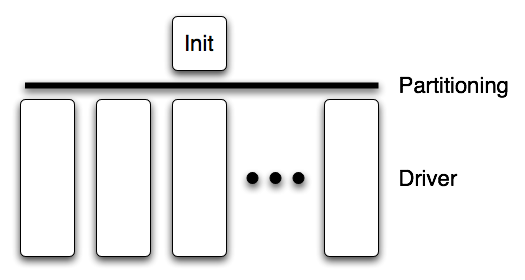
\includegraphics[height=3in]{fig/parfum_structure}
\end{center}
\caption{A typical ParFUM program consists of an {\tt init()} function running in serial context and a {\tt driver()} function running in parallel context.}
\label{fig:parfum_structure}
\end{figure}

In pseudocode, a simple ParFUM program would have the following structure:

\begin{alltt}
     subroutine init
          read the serial mesh and configuration data
     end subroutine
/* after init, the FEM framework partitions the mesh */
     subroutine driver
          get local mesh chunk
          time loop
               FEM computations
               communicate boundary conditions
               more FEM computations
          end time loop
     end subroutine
\end{alltt}

\subsection{ParFUM Programs without init/driver}

Although ParFUM provides the init/driver structure as a convenience to the programmer, you can write a ParFUM program without using init or driver. This is a more flexible approach, but it is more complicated than an init/driver program.

In pseudocode, a ParFUM program with a stand-alone main function might look like this:

\begin{alltt}
   main program
      MPI_Init
      FEM_Init(MPI_COMM_WORLD)
      if (I am master processor)
         read mesh
      partition mesh
      time loop
          FEM computations
          communicate boundary conditions
          more FEM computations
      end time loop
   end main program
\end{alltt}


In this mode, the FEM framework does not set a default reading or writing mesh, and does no partitioning; you must use the FEM\_Mesh routines to create and 
partition your mesh. See the AMPI manual for details on how to declare
the main routine, or the file main.C in ParFUM for an example of how to write a stand-alone main routine. Compiling a ParFUM program without init or driver requires slightly different link flags than a typical ParFUM program, see the compilation section for details.


\subsection{Compilation}

To compile and link a ParFUM program, you must first have a working copy of \charmpp\ and the ParFUM libraries. The process for downloading and building this software is described in section \ref{sec:getting_parfum}.

To compile a FEM program, compile and link using {\tt charmc}, and pass the flag {\tt -language ParFUM}} to charmc when linking. If your program uses its own {\tt main} function rather than init and driver, pass {\tt -language AMPI} instead.

\subsection{Execution}

At runtime, a Charm++/FEM framework program accepts the following
options, in addition to all the usual Charm++ options described in 
the Charm++ ``Installation and Usage Manual''.

\begin{itemize}

\item {\tt +vp} $v$  

Create $v$ mesh chunks, or ``virtual processors''.
By default, the number of mesh chunks is equal to the number of 
physical processors (set with {\tt +p} $p$).


\item {\tt -write}

Skip \kw{driver()}.
After running \kw{init()} normally, the framework partitions the mesh, 
writes the mesh partitions to files, and exits.  As usual, the
{\tt +vp} $v$ option controls the number of mesh partitions.

This option is only used in programs with an {\tt init} function.

\item {\tt -read}

Skip \kw{init()}.
The framework reads the partitioned input mesh from files
and calls \kw{driver()}.  Together with {\tt -write}, this option
allows you to separate out the mesh preparation and partitioning 
phase from the actual parallel solution run.

This can be useful, for example, if \kw{init()} requires more memory 
to hold the unpartitioned mesh than is available on one processor of 
the parallel machine.  To avoid this limitation, you can run the program
with {\tt -write} on a machine with a lot of memory to prepare the input
files, then copy the files and run with {\tt -read} on a machine with 
a lot of processors.

{\tt -read} can also be useful during debugging or performance tuning, 
by skipping the (potentially slow) mesh preparation phase.
This option is only used in programs with a {\tt driver} function.

\item {\tt +tcharm\_trace fem}

Give a diagnostic printout on every call into the ParFUM framework.
This can be useful for locating a sudden crash, or understanding
how the program and framework interact.  Because printing the 
diagnostics can slow a program down, use this option with care.

\end{itemize}